\documentclass[11pt,draftnofoot,onecolumn]{IEEEtran}

\def\spacingset#1{\def\baselinestretch{#1}\small\normalsize}

%\def\ninept{\def\baselinestretch{.95}\let\normalsize\small\normalsize}

\setlength{\topmargin}{-0.4in}             % Move the top margin up with the negative value.
\setlength{\textheight}{9.0in}                % Set the hight of the text.
\setlength{\textwidth}{6.9in}               % Set the width of the text.
\setlength{\oddsidemargin}{-0.2in}           % Set the odd side left margin; useful for the double-sided case.
\setlength{\evensidemargin}{-0.2in}

%\parskip=1pt
\usepackage{amssymb}
\usepackage{amsmath}
\usepackage{latexsym}
\usepackage{epsf}
%\usepackage{psfig}
\usepackage{graphicx}
%\usepackage{showkeys}
%------------------------------------------------------------------
%common definition file for Latex
%------------------------------------------------------------------

\def\bg{\Large}

%------------------------------------------------------------------
% Command for spacing:---------------------------------------------
\def\spacingset#1{\def\baselinestretch{#1}\small\normalsize}
\newcommand{\vs}{\vspace}
\newcommand{\hs}{\hspace}

%------------------------------------------------------------------
% Notations used in linear circuits and electronic devices:--------
\newcommand{\volt}{\, \mbox{V}}
\newcommand{\amp}{\, \mbox{A}}
\newcommand{\mamp}{\, \mbox{mA}}
\newcommand{\ohm}{\, \Omega}
\newcommand{\kohm}{\, \mbox{k}\Omega}
\newcommand{\watt}{\, \mbox{W}}
\newcommand{\kwatt}{\, \mbox{kW}}
\newcommand{\farad}{\, \mbox{F}}
\newcommand{\ufarad}{\, \mu\mbox{F}}
\newcommand{\henry}{\, \mbox{H}}
\newcommand{\mhenry}{\, \mbox{mH}}
\newcommand{\uhenry}{\, \mu\mbox{H}}
\newcommand{\rads}{\, \mbox{rads/s}}


%------------------------------------------------------------------
% Notations for typesetting 'problem' and 'sulution':--------------
\newcommand{\prob}{\noindent {\bf Problem: }}
\newcommand{\soln}{\vspace{0.2cm}\noindent {\bf Solution: }}
\newcommand{\eop}{\hfill $\Box$}

%------------------------------------------------------------------
% Theorem-like environments (defs, lemmas numbered like Theorems):-
\newtheorem{theorem}{Theorem}[section]
\newtheorem{defn}{Definition}[section]
\newtheorem{expl}{Example}[section]

%------------------------------------------------------------------
% Commands for numbering problems:---------------------------------
\newcounter{parnum}
\newcommand{\paraN}[1]{%
    \noindent\refstepcounter{parnum}%
    \rm{#1}\rm{\arabic{parnum}.}}
\newcommand{\paraNb}[1]{%
    \noindent\refstepcounter{parnum}%
    \textbf{#1}\textbf{\arabic{parnum}.}}
%    \makebox[\parindent][l]{\textbf{#1}\textbf{\arabic{parnum}.}}}
%\setlength{\parindent}{2em}

%------------------------------------------------------------------
% Abbreviated commands for equations/listing:----------------------
\newcommand{\ba}{\begin{array}}
\newcommand{\ea}{\end{array}}
\newcommand{\be}{\begin{displaymath}}
\newcommand{\ee}{\end{displaymath}}
\newcommand{\ben}{\begin{equation}}
\newcommand{\een}{\end{equation}}
\newcommand{\bena}{\begin{eqnarray}}
\newcommand{\eena}{\end{eqnarray}}
\newcommand{\beqa}{\begin{eqnarray*}}
\newcommand{\enqa}{\end{eqnarray*}}
\newcommand{\f}{\frac}
\newcommand{\bc}{\begin{center}}
\newcommand{\ec}{\end{center}}
\newcommand{\bi}{\begin{itemize}}
\newcommand{\ei}{\end{itemize}}
\newcommand{\benu}{\begin{enumerate}}
\newcommand{\eenu}{\end{enumerate}}
\newcommand{\bdes}{\begin{description}}
\newcommand{\edes}{\end{description}}
\newcommand{\bt}{\begin{tabular}}
\newcommand{\et}{\end{tabular}}
\newcommand{\sort}{\rm sort \,}
\newcommand{\ds}{\displaystyle}

%------------------------------------------------------------------
% Math symbols:----------------------------------------------------
\newcommand{\tr}{\mathop{\rm tr}}
\newcommand{\var}{\mathop{\rm var}}
\newcommand{\cov}{\mathop{\rm cov}}
\newcommand{\diag}{\mathop{\rm diag}}
\def\rank{\mathop{\rm rank}\nolimits}
\newcommand{\ra}{\rightarrow}
\newcommand{\ul}{\underline}
\def\Pr{\mathop{\rm Pr}}
\def\Re{\mathop{\rm Re}}
\def\Im{\mathop{\rm Im}}
\newcommand{\re}{{\rm Re} \, }
\newcommand{\e}{{\rm E} \, }
\newcommand{\p}{{\rm P} \, }
\newcommand{\cn}{{\cal CN} \, }
\newcommand{\n}{{\cal N} \, }
\newcommand \Cset{{\cal C}}
\newcommand \Rset{{\cal R}}
\newcommand \Zset{{\cal Z}}
\newcommand{\otheta}{\stackrel{\circ}{\theta}}
\newcommand{\defeq}{\stackrel{\bigtriangleup}{=}}
\newcommand{\oabf}{{\bf \breve{a}}}
\newcommand{\odbf}{{\bf \breve{d}}}
\newcommand{\oDbf}{{\bf \breve{D}}}
\newcommand{\oAbf}{{\bf \breve{A}}}
\renewcommand \vec{{\mbox{vec}}}
\newcommand{\Acalbf}{\bf {\cal A}}
\newcommand{\calZbf}{\mbox{\boldmath $\cal Z$}}
\newcommand{\feop}{\hfill \rule{2mm}{2mm} \\}
\newcommand{\Rnum}{{\mathbb R}}
\newcommand{\Cnum}{{\mathbb C}}
\newcommand{\Znum}{{\mathbb Z}}
\newcommand{\Ccal}{{\cal C}}
\newcommand{\Dcal}{{\cal D}}
\newcommand{\Hcal}{{\cal H}}
\newcommand{\Ocal}{{\cal O}}
\newcommand{\Rcal}{{\cal R}}
\newcommand{\Zcal}{{\cal Z}}
\newcommand{\Xcal}{{\cal X}}
\newcommand{\zzbf}{{\bf 0}}
\newcommand{\zebf}{{\bf 0}}
%\newcommand{\gss}{\mathop{}\limits}
\newcommand{\gs}{\mathop{\gss_<^>}\limits} %usage $$\gs_{H_1}^{H_0}$
\newcommand{\circlambda}{\mbox{$\Lambda$
             \kern-.88em\raise1.5ex
             \hbox{$\scriptstyle{\circ}$}}\,}
\def\submbox#1{_{\mbox{\footnotesize #1}}}
\def\supmbox#1{^{\mbox{\footnotesize #1}}}

\makeatletter
\def\revddots{\mathinner{\mkern1mu\raise\p@
\vbox{\kern7\p@\hbox{.}}\mkern2mu
\raise4\p@\hbox{.}\mkern2mu\raise7\p@\hbox{.}\mkern1mu}} \makeatother

%------------------------------------------------------------------
% Bold face symbols:-----------------------------------------------
\newcommand \thetabf{{\mbox{\boldmath$\theta$\unboldmath}}}
\newcommand{\Phibf}{\mbox{${\bf \Phi}$}}
\newcommand{\Psibf}{\mbox{${\bf \Psi}$}}
\newcommand \alphabf{\mbox{\boldmath$\alpha$\unboldmath}}
\newcommand \betabf{\mbox{\boldmath$\beta$\unboldmath}}
\newcommand \gammabf{\mbox{\boldmath$\gamma$\unboldmath}}
\newcommand \deltabf{\mbox{\boldmath$\delta$\unboldmath}}
\newcommand \epsilonbf{\mbox{\boldmath$\epsilon$\unboldmath}}
\newcommand \zetabf{\mbox{\boldmath$\zeta$\unboldmath}}
\newcommand \etabf{\mbox{\boldmath$\eta$\unboldmath}}
\newcommand \iotabf{\mbox{\boldmath$\iota$\unboldmath}}
\newcommand \kappabf{\mbox{\boldmath$\kappa$\unboldmath}}
\newcommand \lambdabf{\mbox{\boldmath$\lambda$\unboldmath}}
\newcommand \mubf{\mbox{\boldmath$\mu$\unboldmath}}
\newcommand \nubf{\mbox{\boldmath$\nu$\unboldmath}}
\newcommand \xibf{\mbox{\boldmath$\xi$\unboldmath}}
\newcommand \pibf{\mbox{\boldmath$\pi$\unboldmath}}
\newcommand \rhobf{\mbox{\boldmath$\rho$\unboldmath}}
\newcommand \sigmabf{\mbox{\boldmath$\sigma$\unboldmath}}
\newcommand \taubf{\mbox{\boldmath$\tau$\unboldmath}}
\newcommand \upsilonbf{\mbox{\boldmath$\upsilon$\unboldmath}}
\newcommand \phibf{\mbox{\boldmath$\phi$\unboldmath}}
\newcommand \varphibf{\mbox{\boldmath$\varphi$\unboldmath}}
\newcommand \chibf{\mbox{\boldmath$\chi$\unboldmath}}
\newcommand \psibf{\mbox{\boldmath$\psi$\unboldmath}}
\newcommand \omegabf{\mbox{\boldmath$\omega$\unboldmath}}
\newcommand \Sigmabf{\hbox{$\bf \Sigma$}}
\newcommand \Upsilonbf{\hbox{$\bf \Upsilon$}}
\newcommand \Omegabf{\hbox{$\bf \Omega$}}
\newcommand \Deltabf{\hbox{$\bf \Delta$}}
\newcommand \Gammabf{\hbox{$\bf \Gamma$}}
\newcommand \Thetabf{\hbox{$\bf \Theta$}}
\newcommand \Lambdabf{\hbox{$\bf \Lambda$}}
\newcommand \Xibf{\hbox{\bf$\Xi$}}
\newcommand \Pibf{\hbox{\bf$\Pi$}}
\newcommand \abf{{\bf a}}
\newcommand \bbf{{\bf b}}
\newcommand \cbf{{\bf c}}
\newcommand \dbf{{\bf d}}
\newcommand \ebf{{\bf e}}
\newcommand \fbf{{\bf f}}
\newcommand \gbf{{\bf g}}
\newcommand \hbf{{\bf h}}
\newcommand \ibf{{\bf i}}
\newcommand \jbf{{\bf j}}
\newcommand \kbf{{\bf k}}
\newcommand \lbf{{\bf l}}
\newcommand \mbf{{\bf m}}
\newcommand \nbf{{\bf n}}
\newcommand \obf{{\bf o}}
\newcommand \pbf{{\bf p}}
\newcommand \qbf{{\bf q}}
\newcommand \rbf{{\bf r}}
\newcommand \sbf{{\bf s}}
\newcommand \tbf{{\bf t}}
\newcommand \ubf{{\bf u}}
\newcommand \vbf{{\bf v}}
\newcommand \wbf{{\bf w}}
\newcommand \xbf{{\bf x}}
\newcommand \ybf{{\bf y}}
\newcommand \zbf{{\bf z}}
\newcommand \rbfa{{\bf r}}
\newcommand \xbfa{{\bf x}}
\newcommand \ybfa{{\bf y}}
\newcommand \Abf{{\bf A}}
\newcommand \Bbf{{\bf B}}
\newcommand \Cbf{{\bf C}}
\newcommand \Dbf{{\bf D}}
\newcommand \Ebf{{\bf E}}
\newcommand \Fbf{{\bf F}}
\newcommand \Gbf{{\bf G}}
\newcommand \Hbf{{\bf H}}
\newcommand \Ibf{{\bf I}}
\newcommand \Jbf{{\bf J}}
\newcommand \Kbf{{\bf K}}
\newcommand \Lbf{{\bf L}}
\newcommand \Mbf{{\bf M}}
\newcommand \Nbf{{\bf N}}
\newcommand \Obf{{\bf O}}
\newcommand \Pbf{{\bf P}}
\newcommand \Qbf{{\bf Q}}
\newcommand \Rbf{{\bf R}}
\newcommand \Sbf{{\bf S}}
\newcommand \Tbf{{\bf T}}
\newcommand \Ubf{{\bf U}}
\newcommand \Vbf{{\bf V}}
\newcommand \Wbf{{\bf W}}
\newcommand \Xbf{{\bf X}}
\newcommand \Ybf{{\bf Y}}
\newcommand \Zbf{{\bf Z}}
\newcommand \Omegabbf{{\bf \Omega}}
\newcommand \Rssbf{{\bf R_{ss}}}
\newcommand \Ryybf{{\bf R_{yy}}}

\newcommand{\fs}{\hspace{0.07in}}   % \fs and \bs will not be used in
\newcommand{\bs}{\hspace{-0.1in}}   % new docs.


%\pagestyle{empty}

%\date{}
%\pssilent
\begin{document}

\spacingset{1.18}


\title{Channel Estimation for an OFDM-Based\\
MIMO System}
%\ninept%
%
%\spacingset{1.127}
\author{\IEEEauthorblockN{Jianhua Liu}
\IEEEauthorblockA{Department of Electrical and Systems Engineering\\
Embry-Riddle Aeronautical University\\
Daytona Beach, FL 32114\\
Email: Jianhua.Liu@erau.edu} %
\and \IEEEauthorblockN{Jian Li}
\IEEEauthorblockA{Department of Electrical and Computer Engineering\\
P.O. Box 116130\\
University of Florida\\
Gainesville, FL 32611-6130}%
}
%
%
\maketitle%
%

\begin{abstract}%
We consider the problem of channel estimation for an orthogonal
frequency-division multiplexing (OFDM)-based multiple-input
multiple-output (MIMO) wireless local area network system. We show
that an existing channel estimation approach, which is based on a
sub-carrier level orthogonal training symbol design and the finite
impulse response channel model, can suffer from severe performance
degradations for realistic OFDM channels. As such, we propose a new
channel estimation approach, which employs a modified version of
this training symbol design and a polynomial fitting/interpolation
method. Our simulation results show that our new channel estimation
approach significantly outperforms the existing one for the
realistic OFDM channels.
\end{abstract}

\vspace{0.2cm}

{\bf Index Terms}---Channel estimation, OFDM, MIMO system, Wireless
LAN standards.


\section{Introduction}
\label{sec1}

Orthogonal frequency-division multiplexing
(OFDM) has been selected as the basis for
several similar new high-speed
wireless local area network (WLAN) standards
\cite{NeeAwaterMorikura1999},
including IEEE 802.11a,
IEEE 802.11g, and HIPERLAN/2, which support a data rate
up to 54 Mbps.
Future WLAN standards, such as the IEEE 802.11n \cite{Coffey2003},
need to support transmission data rates higher than 54 Mbps.
One promising way of increasing the transmission data
rate is to deploy multiple antennas at both the transmitter and
receiver ends to exploit the
huge channel capacity offered by such a system in a multipath-rich
environment. % \cite{FoschiniGans1998,Telatar1999}.
The corresponding system is referred to as
a multiple-input multiple-output (MIMO) WLAN
system. Several OFDM-based
MIMO WLAN systems have been proposed for the multipath-rich,
time-invariant, and frequency-selective fading channels;
see, e.g., \cite{vanZelstSchenk2004,LiuLi2003c}
and the references therein.
Channel response estimation is important for these systems,
and it is usually performed based on training.

In this paper, we consider the training-based {channel response}
estimation for the OFDM-based MIMO system described in
\cite{LiuLi2003c}, which has $M = 2$ transmit antennas and $N = 2$
($N$ can be larger than 2) receive antennas (this system is referred
to as the MIMO system for short in the sequel). A large number of
training-based channel response estimation approaches have been
proposed for systems like the one considered herein. The training
symbols for a majority of these approaches can be casted into two
classes: Class I---sub-carrier level orthogonal training symbols
(see, e.g., \cite{LarssonLi2001,LiYe2002}) and Class II---symbol
level orthogonal training symbols (see, e.g.,
\cite{vanZelstSchenk2004,LiuLi2003c}).

For systems with Class I training symbols,
one transmit antenna (denoted as Tx 1) uses one half of all the sub-carriers
appropriated for training and the other (denoted as Tx 2) uses the remaining half,
and the transmissions from the two transmit antennas
do not interfere with each other---the training symbols from the
two transmit antennas are orthogonal
to each other at the sub-carrier level.
The Class I training symbols were proposed based on the assumption
that an OFDM channel
can be represented by a finite impulse response (FIR) filter,
and a maximum-likelihood (ML)
estimation method is used with these symbols
to estimate the FIR channel response in
time domain; see \cite{LarssonLi2001} for such an existing channel
estimation approach, which is referred to as the ML-FIR approach herein.
An advantage of ML-FIR is that the accompanying Class I training symbols
can be of the same length as those for a single-input single-output
(SISO) %\footnote{The same is true for a single-input multiple-output
%(SIMO) system, which we still refer to SISO system for convenience.}
system. Yet, as pointed out in \cite{BeekEdforsSandell1995,LiuLi2004},
the FIR channel model is
only a poor approximation of the realistic OFDM channels.
For the realistic OFDM channels, channel estimates obtained from
approaches such as ML-FIR suffer from severe
performance degradations.

For systems with Class II training symbols,
each transmit antenna uses all the sub-carriers appropriated
for training, and the transmissions from the two transmit antennas
are separated using on/off transmission (see, e.g., \cite{vanZelstSchenk2004})
or plus/minus transmission (see, e.g., \cite{LiuLi2003c})---the training
symbols are orthogonal to each other at the symbol level.
An advantage of using Class II training symbols is that
the simple sub-carrier training method,
which is the same as for the SISO case \cite{LiuLi2004},
can be used for channel response
estimation in frequency domain (FD), which can obviate
the necessity of the FIR model assumption.
Yet, the length of the Class II training symbols
is usually twice as long as that for a SISO
system, and hence has a larger overhead.

Our focus herein is to improve the overhead/channel estimation performance
trade-offs for the MIMO system. We propose a new channel estimation
approach, which is based on a modified version
of the Class I training symbols.
The new approach, which exploits the polynomial approximation \cite{WangLiu2002}
of the FD channel response,
is referred to as the polynomial fitting/interpolation (PF/I)
approach. PF/I estimates channel response in FD
by first applying polynomial fitting to the sub-carriers
containing the training symbols and then performing interpolation to
cover the sub-carriers
without training symbols.
Our simulation results show that PF/I
can significantly outperform
ML-FIR for realistic OFDM channels.
This suggests that the polynomial model is superior to the
FIR model for channel response estimation for the OFDM signaling.

%\vspace{-0.2cm}
\section{Background}
\label{sec2}

Before describing the background for the MIMO channel response
estimation---the MIMO preamble and channel model---we first
give an overview of the IEEE 802.11a standard, based on
which the MIMO system is designed.


\subsection{Overview of IEEE 802.11a}

%Figure \ref{fig_ofdmpacket} shows the IEEE 802.11a packet structure.
%In this case,
%the number of samples $N_S = 64$ for a data OFDM symbol is equal to
%the number of sub-carriers.
The OFDM packet preamble of a SISO system, as shown in Fig. \ref{fig_ofdmpacket}(a),
consists of 10 identical short OFDM training
symbols ${\rm t}_i, i = 1, 2, \dots, 10$, each of which contains
$N_C = 16$ samples, and 2 identical long
OFDM training symbols ${\rm T}_i, i = 1, 2$, each of which contains
$N_S = 64$ samples.
(The nominal bandwidth of the OFDM signal is 20 MHz and
the in-phase/quadrature sampling interval $t_S$ is 50 ns.)
Between the short and long OFDM training symbols there is a
long guard interval (GI2) consisting of $2N_C = 32$ data samples, which
is the cyclic prefix (CP) for ${\rm T}_1$.
The long training symbols can be used to estimate the SISO
channel response.

\begin{figure*}[t]
\centering
\begin{tabular}{c}
%{\psfig{figure=fig/ofdmpacket_n.eps,height=0.8in}}\\
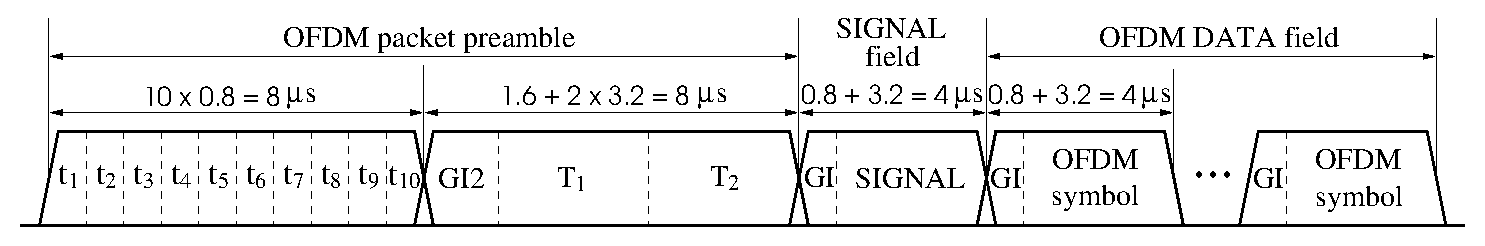
\includegraphics[height=0.8in]{fig/ofdmpacket_n.eps} \\
{\small (a)}\\
%{\psfig{figure=fig/mimopac_short_t.eps,height=0.8in}}\\
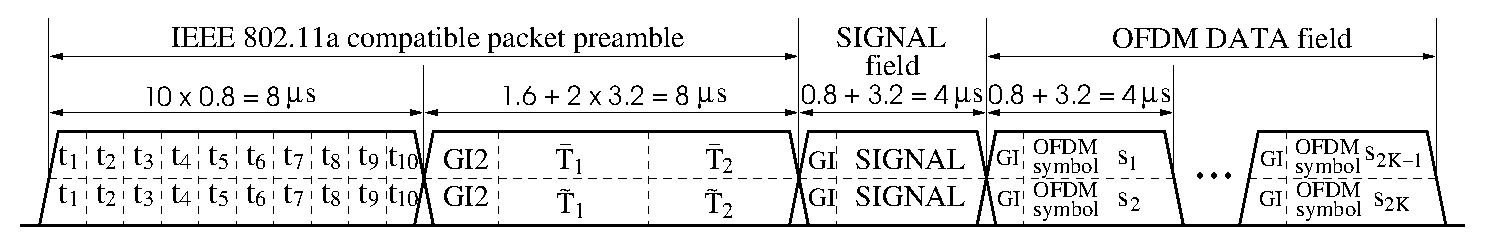
\includegraphics[height=0.8in]{fig/mimopac_short_t.eps} \\
{\small (b)}
\end{tabular}
\caption{Packet structure for the OFDM-based WLANs: (a) an
IEEE 802.11a conformable SISO system and (b) the MIMO system.}
\label{fig_ofdmpacket}
\end{figure*}

The information carrying data are encoded in the OFDM DATA field.
%The binary source data sequence is first scrambled and then Convolutionally
%enCoded (CC) by an industrial standard
%rate 1/2 encoder. The CC encoded output is then
%punctured according to the data rate requirement and is
%segmented into blocks of length $N_{\rm CBPS}$,
%each of which corresponds to an
%OFDM data symbol. The binary data in each block is first interleaved
%among the sub-carriers and then mapped into QAM
%symbols, which are used to modulate the different data carrying sub-carriers.
Each OFDM data symbol employs $N_S = 64$ sub-carriers,
52 of which are used for data or
pilot symbols. There are also 12 null sub-carriers
with one in the center and the other 11 on the two
ends of the frequency band.
The OFDM data symbols
are obtained via taking IFFT
of the data symbols, pilot symbols, and nulls on these $N_S$ sub-carriers.
To eliminate the
inter-symbol interference, each OFDM data symbol is
preceded by a CP or guard interval (GI) containing the
last $N_C$ samples of the OFDM data symbol.

\subsection{MIMO Preamble with Modified Class I Training Symbols}

For the MIMO system considered herein,
two packets, with corresponding preambles,
are transmitted simultaneously from Tx 1 and Tx 2.
To be backward compatible with the SISO preamble,
the same short training symbols as in the
SISO one are used for both Tx 1 and Tx 2. However, the
long training symbols cannot be used directly.

The Class I training symbols, i.e., the long OFDM training symbols
for the MIMO system, are obtained by first splitting
orthogonally \cite{LarssonLi2001,LiYe2002}
the original IEEE 802.11a FD training sequence,
denoted by x's, to obtain two training sequences with
zeros inserted at appropriate places, as shown in Table \ref{tab_preamble},
and then taking IFFTs of the two training sequences.
Note that we have modified the Class I training symbols by
adding two additional training bits, each at one end of
the bandwidth, to improve the channel estimation performance.
%(We use the same total transmission power as for IEEE 802.11a.)
Let the corresponding time-domain (TD) training symbols for
Tx 1 and Tx 2 be denoted as $\bar{\rm T}_1$ and $\tilde{\rm T}_1$, respectively,
and let $\bar{\rm T}_2 = \bar{\rm T}_1$ and $\tilde{\rm T}_2 = \tilde{\rm T}_1$.
Then we have the MIMO preamble design,
as shown in Fig. \ref{fig_ofdmpacket}(b).
The MIMO preamble with the modified Class I training symbols
is shorter than the one given in \cite{LiuLi2003c},
which was designed to be IEEE 802.11a backward compatible,
and hence the former has a smaller overhead than the latter.
%We remark that although the bandwidth of the new MIMO preamble is slightly
%wider than before, is will not have noticeable impact on the system
%operation, due to the bandwidth protection tolerance
%allowed in the IEEE 802.11a standard.
Note that
the design in Fig. \ref{fig_ofdmpacket}(b) is also backward compatible with
IEEE 802.11a since exactly the same FD training sequence as
IEEE 802.11a is transmitted on the original 52 sub-carriers and the
two additional sub-carriers can be discarded automatically
by the SISO system.

\begin{table*}[t]
\caption{FD training sequences for the modified Class I training
symbols for the MIMO system.}
\label{tab_preamble}
\centering
{\small
\begin{tabular}{r|ccccccccccccccc}
$[n_S-1]_{N_S}$ & $-27$ & $-26$ & $-25$ & $-24$ & ... & $-2$ & $-1$ & 0 & 1 & 2 & ... & 24 & 25 & 26 & 27 \\ \hline
Tx 1 & $-1$ & 0  & x  & 0   & ... & 0  & x  & 0 & 0 & x & ... & x  & 0  & x & 0\\
Tx 2 & 0 & x  & 0  & x    & ... & x  & 0  & 0 & x & 0 & ... & 0  & x  & 0 & $-1$
\end{tabular}
}
\end{table*}

\subsection{Realistic OFDM Channel Model}

For the SISO system, the TD channel response is sometimes modeled by
an exponentially decaying FIR filter with length $L_F$%
\ben %
h_e (t)
= \sum_{l_F=0}^{L_F -1} h^{\rm (t)}_{l_F} \delta (t - l_F t_S ),%
\label{equ_ch_model2} %
\een %
where %
\ben %
h_{l_F}^{(\rm t)} \sim \n
\left ( 0, \left ( 1 - e^{-1/t_n} \right )
   e^{-l_F/t_n} \right )%
\label{equ_fir_hl}%
\een%
(zero-mean Gaussian) with $ \left \{ h_{l_F}^{(\rm t)} \right
\}_{l_F = 0}^{L_F-1}$ being independent of each other, $t_n = t_r /
t_S$, $t_r$ being the root-mean-square delay spread of the
frequency-selective fading channel, $L_F = \lceil 10 t_n \rceil +
1$, and $\lceil x \rceil$ denoting the smallest integer not less
than $x$. % \cite{Chayat1997}.
While the FIR model is convenient for simulation purposes, it simulates only
a very special case of the true OFDM channel, where the time
delays are constrained to the multiples of the  sampling instants
\cite{BeekEdforsSandell1995,LiuLi2004}.

We modify (\ref{equ_ch_model2}) slightly to obtain a {\em generic}
model for realistic OFDM channels as %
\ben %
h_m (t) =
\sum_{l_F=0}^{L_F -1} h^{\rm (t)}_{l_F} \delta(t - l_F t_S -
t_{l_F}), %
\label{equ_ch_model3} %
\een %
where for $l_F = 0, 1, \dots,
L_F-1$, the multipath gain $h^{\rm (t)}_{l_F}$ is as in
(\ref{equ_fir_hl}) and the time delay $t_{l_F}$ is uniformly
distributed over $[0, t_S]$. We also assume that $ \left \{
h_{l_F}^{(\rm t)} \right \}_{l_F = 0}^{L_F-1}$ and $ \left \{
t_{l_F} \right \}_{l_F = 0}^{L_F-1}$ are independent of each other.
The channel model in (\ref{equ_ch_model3}) is more realistic than
the one in (\ref{equ_ch_model2}) due to the flexible time delays $
\left \{ t_{l_F} \right \}_{l_F = 0}^{L_F-1}$ introduced in
(\ref{equ_ch_model3}).

Consider the base-band processing and an ideal low-pass filtering
before A/D conversion at the receiver. The corresponding FD channel
response (also called channel gain) of (\ref{equ_ch_model3}) on
sub-carrier $n_S$, $n_S = 1, 2, \dots, N_S$, is then given by%
\ben%
{h}_{n_S} = \sum_{l_F = 0}^{L_F - 1} h_{l_F}^{\rm (t)} e^{-j 2 \pi
\frac{l_F t_S + t_{l_F}}{N_S t_S} [n_S-1]_{N_S} },%
\label{equ_fre_h_n_S} %
\een %
where $[n_S - 1]_{N_S}$ is equal to
$n_S-1$ for $n_S \le N_S/2$ and $n_S-1-N_S$ for $n_S > N_S/2$.

For the MIMO system, each channel can be
modeled by (\ref{equ_ch_model3}).
For path $l_F$, $l_F = 0, 1, \dots, L_F-1$, the path gains
for the MIMO channels are assumed to be independent of each other (correlations
can be easily added), whereas the time delays are
assumed the same for all the channels.

\section{Channel Estimation}
\label{sec3}

For the MIMO system, the task of channel estimation is to estimate
the FD channel gain matrix %
\ben {\Hbf} = \left [\ba{cc}
   {h}_{n_S}^{(1,1)} & {h}_{n_S}^{(1,2)} \\
   {h}_{n_S}^{(2,1)} & {h}_{n_S}^{(2,2)} \ea
   \right ] \in {{\mathbb C}}^{2\times 2}
\label{eq_modelofh}
\een
for the 52 data/pilot carrying sub-carriers,
where ${h}_{n_S}^{(n,m)}$ denotes the channel
gain from Tx $m$ to receive antenna (Rx) $n$
on the $n_S$th sub-carrier.

To estimate the channel responses on those sub-carriers without training symbols,
we must exploit the channel correlations among sub-carriers.
One simple way is to resort to channel
models to approximate the OFDM channels. The FIR model of
\cite{LarssonLi2001,LiYe2002} is an example and is widely used.
An alternative model, which we advocate here, is the recently
introduced piecewise polynomial model \cite{WangLiu2002}.
It has been successfully used to improve the channel
response estimation accuracy for SISO OFDM channels.
It is preferred over the FIR counterpart
for realistic OFDM channels
since: (a) the FD channel response of an FIR filter {\em must be
periodic} in $N_S$ (as can be seen in (\ref{equ_fre_h_n_S})
by dropping the $t_{l_F}$'s) whereas
the FD channel response of a realistic OFDM channel
{\em cannot be periodic} unless $t_{l_F} = 0$ for all $l_F$,
which is clear from (\ref{equ_fre_h_n_S}),
and (b) the FD channel response described by a polynomial
{\em can be flexible} (without this periodicity constraint).
%
%We know from (\ref{equ_fre_h_n_S}) that
%the channel gain sequence, in terms of $n_S$,
%is a superposition of multiple complex sinusoids with
%frequencies not constrained on multiples of the normalized
%base frequency $2\pi / N_S$.
%(This is the reason why the FIR model works inferiorly.)
%The complex sinusoid can be approximated by a
%polynomial of $n_S$ with complex coefficients.
%The higher the order of the polynomial, the more accurate the approximation;
%the higher frequency of the complex sinusoid, the higher the order
%of the polynomial needed to maintain the same accuracy.
%
An additional advantage of the polynomial approximation is
that it is not sensitive to the responses of the filters used
at the transmitter and receiver since the effects of these filters
can be easily absorbed into the polynomials.

%\subsection{Channel Estimation}

Consider the estimation of the channels from
Tx 1 and Tx 2 to Rx $n$, $n= 1,2$.
As in \cite{WangLiu2002}, we use piecewise polynomials to
approximate the FD channel responses. We group the sub-carriers
into 4 sets, with each set corresponding to a polynomial.
This grouping depends on the transmit antenna:
for Tx 1, the 4 sets are, respectively, %
\bena%
{\cal S}_{1,1} & \bs = \bs & \{-27, -26, \dots, -13 \}, \nonumber
\\
{\cal S}_{1,2} & \bs = \bs & \{-15, -14, \dots, -1 \}, \nonumber
\\
{\cal S}_{1,3} & \bs = \bs & \{-1, 0, \dots, 14 \}, \nonumber \\
{\cal S}_{1,4} & \bs = \bs & \{12, 13, \dots, 26 \}; \nonumber %
\eena%
and for Tx 2, the 4 sets are, respectively, %
\bena%
{\cal S}_{2,1} & \bs = \bs & \{-26, -25, \dots, -12 \}, \nonumber \\
{\cal S}_{2,2} & \bs = \bs & \{-14, -12, \dots, 1 \}, \nonumber
\\
{\cal S}_{2,3} & \bs = \bs & \{1, 2, \dots, 15 \}, \nonumber \\
{\cal S}_{2,4} & \bs = \bs & \{13, 14, \dots, 27 \}. \nonumber %
\eena %
We remark that the above sets are grouped in such a way that
each set contains 8 sub-carriers with training symbols, as can be
seen from Table I.

A polynomial of order $P$ can be used to approximate the FD channel
response on each of the above sets. For example, for channel
$h_{n_S}^{(n,1)}$ on ${\cal S}_{1,1}$ ($-27 \le [n_S - 1 ]_{N_S} \le
-13$), we have%
\ben h_{n_S}^{(n,1)} = \sum_{p=0}^P
{\alpha}_p^{(n,1,1)}
   \left ( [n_S - 1 ]_{N_S} - f^{(n,1,1)} \right )^p
   + e_{n_S, P}^{(n,1,1)},%
\label{equ_h_poly}%
\een%
where ${\alpha}_p^{(n,1,1)}$, $p=0, 1, \dots, P$, is the $p$th (complex)
polynomial coefficient,
$e_{n_S, P}^{(n,1,1)}$ is the model error depending on $P$
and $f^{(n,1,1)} = -20$ is used to shift the initial location of the polynomial.
(For the above three-letter-superscript indexing,
the first two are used to refer to the
channel between Tx 1 and Rx $n$, and the last two the sub-carrier set.)

Now, let us consider the new PF/I method for the MIMO system by
considering $h_{n_S}^{(n,1)}$ on ${\cal S}_{1,1}$ as an example. Let
$\vbf_1 = [-7 \fs -5 \fs -3 \fs -1 \fs 1 \fs 3 \fs 5 \fs 7]^T$ (with
$T$ denoting the transpose) and $\Vbf_1$ be the $8\times (P+1)$
matrix with the $i$th column being $\vbf^{.(i-1)}_1$ (element-wise
power). Let $\hat{\hbf}_{C}^{(n,1,1)} \in {{\mathbb C}}^{8\times 1}$
be the channel gain estimates on the sub-carriers with training
symbols, i.e., sub-carriers $\{-27, -25, -23, -21, -19, -17, -15,
-13\}$, obtained via sub-carrier training in the same way as for the
SISO system. Then the polynomial coefficients obtained via
polynomial fitting (PF) can be written as%
\begin{eqnarray}
\hat{{\alphabf}}^{(n,1,1)} & \bs = \bs &
   [\hat{\alpha}_0^{(n,1,1)} \fs \hat{\alpha}_1^{(n,1,1)} \fs \dots
   \fs \hat{\alpha}_P^{(n,1,1)} ]^T \nonumber \\
   & \bs = \bs &
   (\Vbf_1^T \Vbf_1 )^{-1} \Vbf_1^T \hat{\hbf}_{C}^{(n,1,1)}.
\label{equ_PF_coe}
\end{eqnarray}
Let $\hat{\hbf}_F^{(n,1,1)}$ be the PF counterpart of
$\hat{\hbf}_{C}^{(n,1,1)}$. Then $\hat{\hbf}_F^{(n,1,1)}$ can be
obtained using %
\ben %
\hat{\hbf}_F^{(n,1,1)}
   = \Vbf_1 \hat{{\alphabf}}^{(n,1,1)}.%
\label{equ_h_PF} %
\een %
Let ${\vbf} = [-6 \fs -4 \fs -2 \fs 0 \fs 2
\fs 4 \fs 6]^T$ and ${\Vbf}$ be the matrix formed from ${\vbf}$ in
the same way as ${\Vbf}_1$ from ${\vbf}_1$. Let
$\hat{\hbf}_I^{(n,1,1)}$ be the channel response estimate on
sub-carriers $\{-26, -24, -23, -20$, $-18, -16, -16\}$ via
polynomial interpolation. Then, we have %
\ben %
\hat{\hbf}_I^{(n,1,1)}
   = {\Vbf} \hat{{\alphabf}}^{(n,1,1)}.
\label{equ_h_PI}
\een
Combining $\hat{\hbf}_F^{(n,1,1)}$ and $\hat{\hbf}_I^{(n,1,1)}$,
we obtain the estimate of the channel response from Tx 1 to Rx $n$ on
${\cal S}_{1,1}$.

In exactly the same way, we can estimate the
channel responses from Tx 1 to Rx $n$ on
${\cal S}_{1,2}$ and ${\cal S}_{1,4}$
as well as those from Tx 2 to Rx $n$ on
${\cal S}_{2,1}$, ${\cal S}_{2,3}$, and ${\cal S}_{2,4}$.
As for channels
from Tx 1 to Rx $n$ on ${\cal S}_{1,3}$
and from Tx 2 to Rx $n$ on ${\cal S}_{2,2}$,
the response can be obtained similarly.
Let $\vbf_2 = [-8 \fs -5, \fs -3 \fs -1 \fs 1 \fs 3 \fs 5 \fs 7]^T$
and ${\Vbf}_2$ be the matrix formed from ${\vbf}_2$ in the
same way as ${\Vbf}_1$ from ${\vbf}_1$.
Let $\hat{{\alphabf}}^{(n,1,3)}$, $\hat{\hbf}_C^{(n,1,3)}$, $\hat{\hbf}_F^{(n,1,3)}$,
and $\hat{\hbf}_I^{(n,1,3)}$ be the counterparts of $\hat{{\alphabf}}^{(n,1,1)}$,
$\hat{\hbf}_C^{(n,1,1)}$, $\hat{\hbf}_F^{(n,1,1)}$,
and $\hat{\hbf}_I^{(n,1,1)}$.
Then we have, corresponding to (\ref{equ_PF_coe}), (\ref{equ_h_PF}),
and (\ref{equ_h_PI}), respectively,%
\bena%
\hat{{\alphabf}}^{(n,1,3)} & \bs = \bs & (\Vbf_2^T \Vbf_2 )^{-1}
\Vbf_2^T \hat{\hbf}_{C}^{(n,1,3)}, \\
\hat{\hbf}_F^{(n,1,3)} & \bs = \bs & \Vbf_2
\hat{{\alphabf}}^{(n,1,3)}, \\
\hat{\hbf}_I^{(n,1,3)} & \bs = \bs & {\Vbf}
\hat{{\alphabf}}^{(n,1,3)}.%
\eena%


\section{Numerical Examples}
\label{sec5}

\begin{figure}[t]
%\vspace{1cm}
\centering
%\begin{tabular}{c}
%%{\psfig{figure=../fig_channel_MSE_MCCM_50ns27sc.eps,height=3.2in}}
%{\psfig{figure=fig/fig_ch_MSE_MCCM_50ns27sc_4p.eps,height=2.6in}}
%\end{tabular}
\includegraphics[height=2.6in]{fig/fig_ch_MSE_MCCM_50ns27sc_4p.eps}
%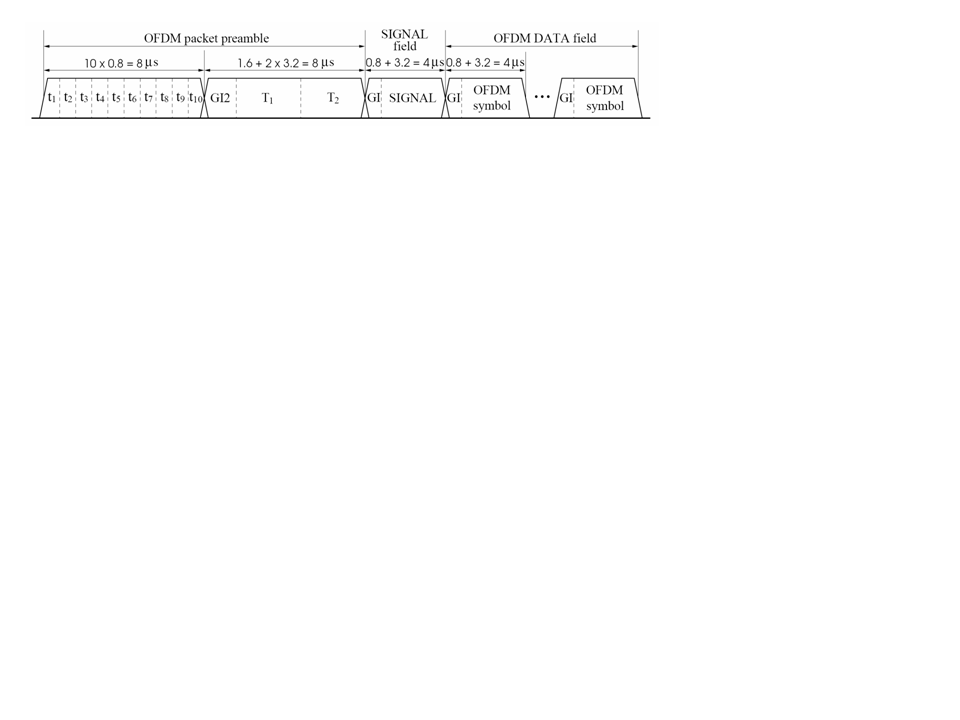
\includegraphics[height=0.6in]{fig/Presentation2.bmp}
\caption{MSE versus $P$ or $4P$ comparison between PF/I and ML-FIR.}
\label{fig_MSE_vs_P}
\end{figure}

\begin{figure}[t]
%\vspace{1cm}
\centering
%\begin{tabular}{c}
%%{\psfig{figure=../fig_PER_SoftLS_108_50ns54sc.eps,height=3.2in}}
%{\psfig{figure=fig/fig_ch_MSE_MCCM_SNR_4p.eps,height=2.6in}}
%\end{tabular}
\includegraphics[height=2.6in]{fig/fig_ch_MSE_MCCM_SNR_4p.eps}
\caption{MSE versus SNR comparison between PF/I and ML-FIR.}
\label{fig_MSE_vs_SNR}
\end{figure}

We provide two numerical examples to demonstrate the performance of
our new channel estimation approach. Due to the fact that 52 out of
64 sub-carriers are used in the OFDM-based WLAN systems, the SNR
used herein is the symbol-to-noise-power ratio normalized by
$52/64$. For a given SNR, we use the same total transmission power
for both the MIMO and SISO systems.

Fig. \ref{fig_MSE_vs_P} shows the
mean-squared-error (MSE) comparison of PF/I
and ML-FIR as a function of
$P$ for the MIMO system with the modified Class I training symbols over
realistic OFDM channels generated according to (\ref{equ_ch_model3})
with $t_r = $ 50 ns and SNR being 20 and 30 dB, respectively.
(For ML-FIR, $P$ is the length of FIR channel.)
Fig. \ref{fig_MSE_vs_SNR} shows the
MSE comparison of PF/I (with $P = 5$)
and ML-FIR ($P=19$) as a function of SNR under the same simulation
conditions as for Fig. \ref{fig_MSE_vs_P}.
We can see from the figures that
our new PF/I approach significantly outperforms
ML-FIR for realistic OFDM channels, especially
at high SNRs which are desired for high data rate MIMO systems
\cite{LiuLi2003c}. This suggests that the polynomial
model is superior to its FIR counterpart
for channel estimation for the OFDM signaling.


\section{Concluding Remarks}
\label{sec6}

We have proposed a new channel estimation approach,
a PF/I method based on a modified Class I training symbol design,
for an OFDM-based MIMO WLAN system.
Simulation results have
shown that the new channel estimation approach can significantly
outperform existing ones.

%\spacingset{1.025}
\bibliographystyle{ieeetr}
\bibliography{../../commonFiles/all}
%\bibliography{C:/Users/jhl/OneDrive/jhltch/senior_design/20_21/citationGraph/commonFiles/all}


\end{document}
